\section{Identification des besoins et de l'environnement du travail}

\subsection{Introduction}
Analyse complète des besoins fonctionnels et non-fonctionnels pour la plateforme ETL Medallion.

\subsection{Analyse fonctionnelle du système}
\subsubsection{Identification des acteurs}
\begin{itemize}
    \item Utilisateurs finaux (analystes financiers)
    \item Administrateurs système
    \item Développeurs et mainteneurs
    \item Utilisateurs de l'IA conversationnelle
\end{itemize}

\subsubsection{Besoins fonctionnels}
\begin{itemize}
    \item Collecte automatisée des données BVMT
    \item Traitement ETL avec architecture Medallion
    \item Analyse prédictive avec modèles avancés
    \item Visualisation interactive des données
    \item Système d'authentification et gestion des utilisateurs
    \item Assistance IA conversationnelle
\end{itemize}

\subsubsection{Besoins non fonctionnels}
\begin{itemize}
    \item Performance : Traitement de grandes volumes de données
    \item Fiabilité : Disponibilité 99.9\%
    \item Sécurité : Protection des données financières sensibles
    \item Scalabilité : Architecture extensible
    \item Maintenabilité : Code modulaire et documenté
\end{itemize}

\subsection{Technologies et outils utilisés}
\subsubsection{Backend}
\begin{itemize}
    \item Python 3.9+ (pandas, numpy, scikit-learn, statsmodels)
    \begin{figure}[H]
    \centering
    
\includegraphics[width=\figwidth]{img/Python 3.9+.png}
    \caption{python}
    \label{fig:python}
\end{figure}
    \item Flask 3.0 (APIs REST)
    \begin{figure}[H]
    \centering
    
\includegraphics[width=\figwidth]{img/Flask 3.0.png}
    \caption{flask}
    \label{fig:flask}
\end{figure}
    \item PostgreSQL (base de données enterprise)
     \begin{figure}[H]
    \centering
    
\includegraphics[width=\figwidth]{img/postsql.png}
    \caption{postsql}
    \label{fig:postsql}
\end{figure}
    
    \item JWT (authentification sécurisée)
     \begin{figure}[H]
    \centering
    
\includegraphics[width=\figwidth]{img/jwtt (1).png}
    \caption{jwt}
    \label{fig:jwt}
\end{figure}
\end{itemize}

\subsubsection{Frontend}
\begin{itemize}
    \item React 19 (JavaScript ES6+)
    \begin{itemize}
    
    \begin{figure}[H]
    \centering
    \includegraphics[width=\figwidth]{img/— React 19.png}
    \caption{React}
    \label{fig:React}
\end{figure}
    \item Tailwind CSS (styling moderne)
     \begin{figure}[H]
    \centering
    \includegraphics[width=\figwidth]{img/— Tailwind CSS (.png}
    \caption{tailwind}
    \label{fig:tailwind}
\end{figure}
    \item Framer Motion (animations)
    \begin{figure}[H]
    \centering
    \includegraphics[width=\figwidth]{img/— Framer Motion.png}
    \caption{framer}
    \label{fig:framer}
\end{figure}
    \item PowerBI (visualisation professionnelle)
    \begin{figure}[H]
    \centering
    
\includegraphics[width=\figwidth]{img/power bu.png}
    \caption{power bi}
    \label{fig:power bi}
\end{figure}
\end{itemize}

\subsubsection{Infrastructure}
\begin{itemize}
    \item Docker (containerisation)
    \begin{figure}[H]
    \centering
    
\includegraphics[width=\figwidth]{img/Docker.png}
    \caption{docker}
    \label{fig:docker}
\end{figure}
    \item Git (versioning)
    \begin{figure}[H]
    \centering
    
\includegraphics[width=\figwidth]{img/Git.png}
    \caption{Git}
    \label{fig:Git}
\end{figure}
    \item Virtual Environment (isolation des dépendances)
\end{itemize}
\begin{figure}[H]
    \centering
    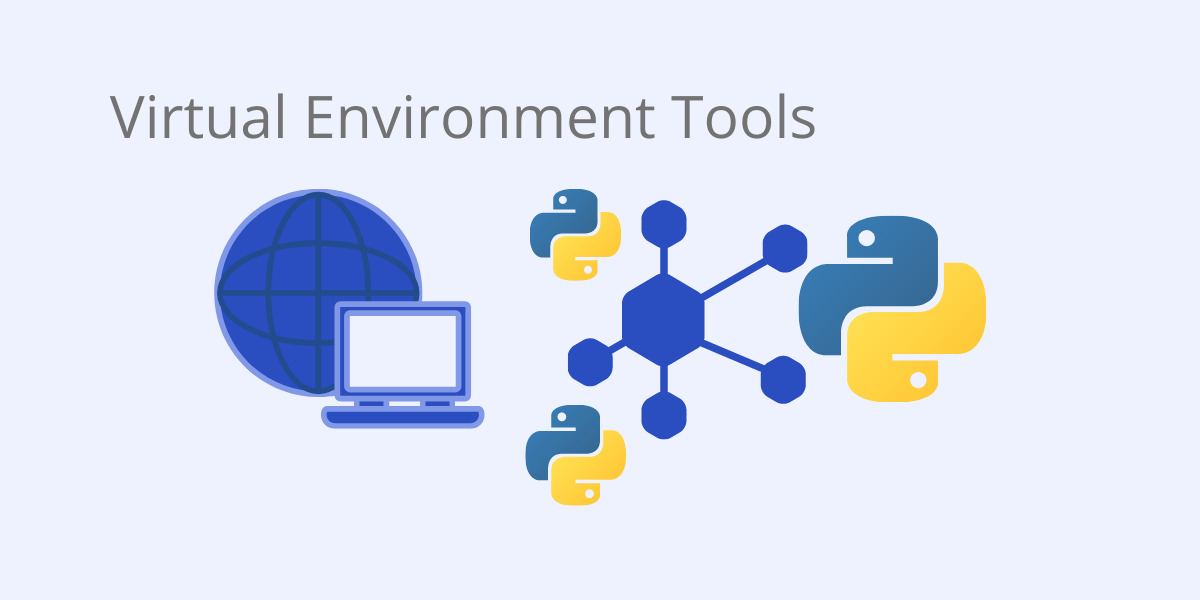
\includegraphics[width=\figwidth]{img/Virtual Environment.jpg}
    \caption{Virtual Environment}
    \label{fig:Virtual Environment}
\end{figure}

